\documentclass[a4paper,12pt]{article} % добавить leqno в [] для нумерации слева
\usepackage[a4paper,top=1.3cm,bottom=2cm,left=1.5cm,right=1.5cm,marginparwidth=0.75cm]{geometry}
%%% Работа с русским языком
\usepackage{cmap}					% поиск в PDF
\usepackage{mathtext} 				% русские буквы в фомулах
\usepackage[T2A]{fontenc}			% кодировка
\usepackage[utf8]{inputenc}			% кодировка исходного текста
\usepackage[english,russian]{babel}	% локализация и переносы

\usepackage{graphicx}

\usepackage{wrapfig}
\usepackage{tabularx}

\usepackage{hyperref}
\usepackage[rgb]{xcolor}
\hypersetup{
colorlinks=true,urlcolor=blue
}

%%% Дополнительная работа с математикой
\usepackage{amsmath,amsfonts,amssymb,amsthm,mathtools} % AMS
\usepackage{icomma} % "Умная" запятая: $0,2$ --- число, $0, 2$ --- перечисление

%% Номера формул
\mathtoolsset{showonlyrefs=true} % Показывать номера только у тех формул, на которые есть \eqref{} в тексте.

%% Шрифты
\usepackage{euscript}	 % Шрифт Евклид
\usepackage{mathrsfs} % Красивый матшрифт

%% Свои команды
\DeclareMathOperator{\sgn}{\mathop{sgn}}

%% Перенос знаков в формулах (по Львовскому)
\newcommand*{\hm}[1]{#1\nobreak\discretionary{}
{\hbox{$\mathsurround=0pt #1$}}{}}

%%% Заголовок
\author{Сенокосов Арсений Олегович}
\title{Лабораторная работа №1.1.1

Измерение удельного сопротивления нихромовой проволоки
}
\date{\today}

\begin{document}

\begin{titlepage}
	\begin{center}
		{\large МОСКОВСКИЙ ФИЗИКО-ТЕХНИЧЕСКИЙ ИНСТИТУТ (НАЦИОНАЛЬНЫЙ ИССЛЕДОВАТЕЛЬСКИЙ УНИВЕРСИТЕТ)}
	\end{center}
	\begin{center}
		{\large Физтех-школа физики и исследований им. Ландау}
	\end{center}
	
	
	\vspace{4.5cm}
	{\huge
		\begin{center}
			{\bf Отчёт о выполнении лабораторной работы 1.1.1}\\
			Определение удельного сопротивления нихромовой проволоки
		\end{center}
	}
	\vspace{2cm}
	\begin{flushright}
		{\LARGE Автор:\\ Сенокосов Арсений Олегович \\
			\vspace{0.2cm}
			Б02-012}
	\end{flushright}
	\vspace{8cm}
	\begin{center}
		Долгопрудный 2020
	\end{center}
\end{titlepage}

\section{Введение}

\textbf{Цель работы:} измерить удельное сопротивление тонкой проволоки круглого сечения, изготовленной из нихромового сплава.
\medskip

\textbf{В работе используются:} линейка, штангенциркуль, микрометр, отрезок проволоки из нихрома, амперметр, вольтметр, источник ЭДС, мост постоянного тока, реостат, ключ.
\medskip

В работе используются следующие методы измерения сопротивления:
\begin{enumerate}
	\item определение углового коэффициента наклона зависимости напряжения на проволоке от тока через неё;
	\item измерение с помощью моста постоянного тока.
\end{enumerate}

\section{Теоретические сведения}

Удельное сопротивления однородной проволоки круглого сечения можно определить по следующей формуле:

\begin{equation}\label{1form}
\rho = R \frac{\pi d^2}{4l},
\end{equation}

\noindent где $R$ -- сопротивление проволоки, $d$ -- её диаметр, $l$ -- длина.

\medskip

\begin{wrapfigure}{r}{7cm}
	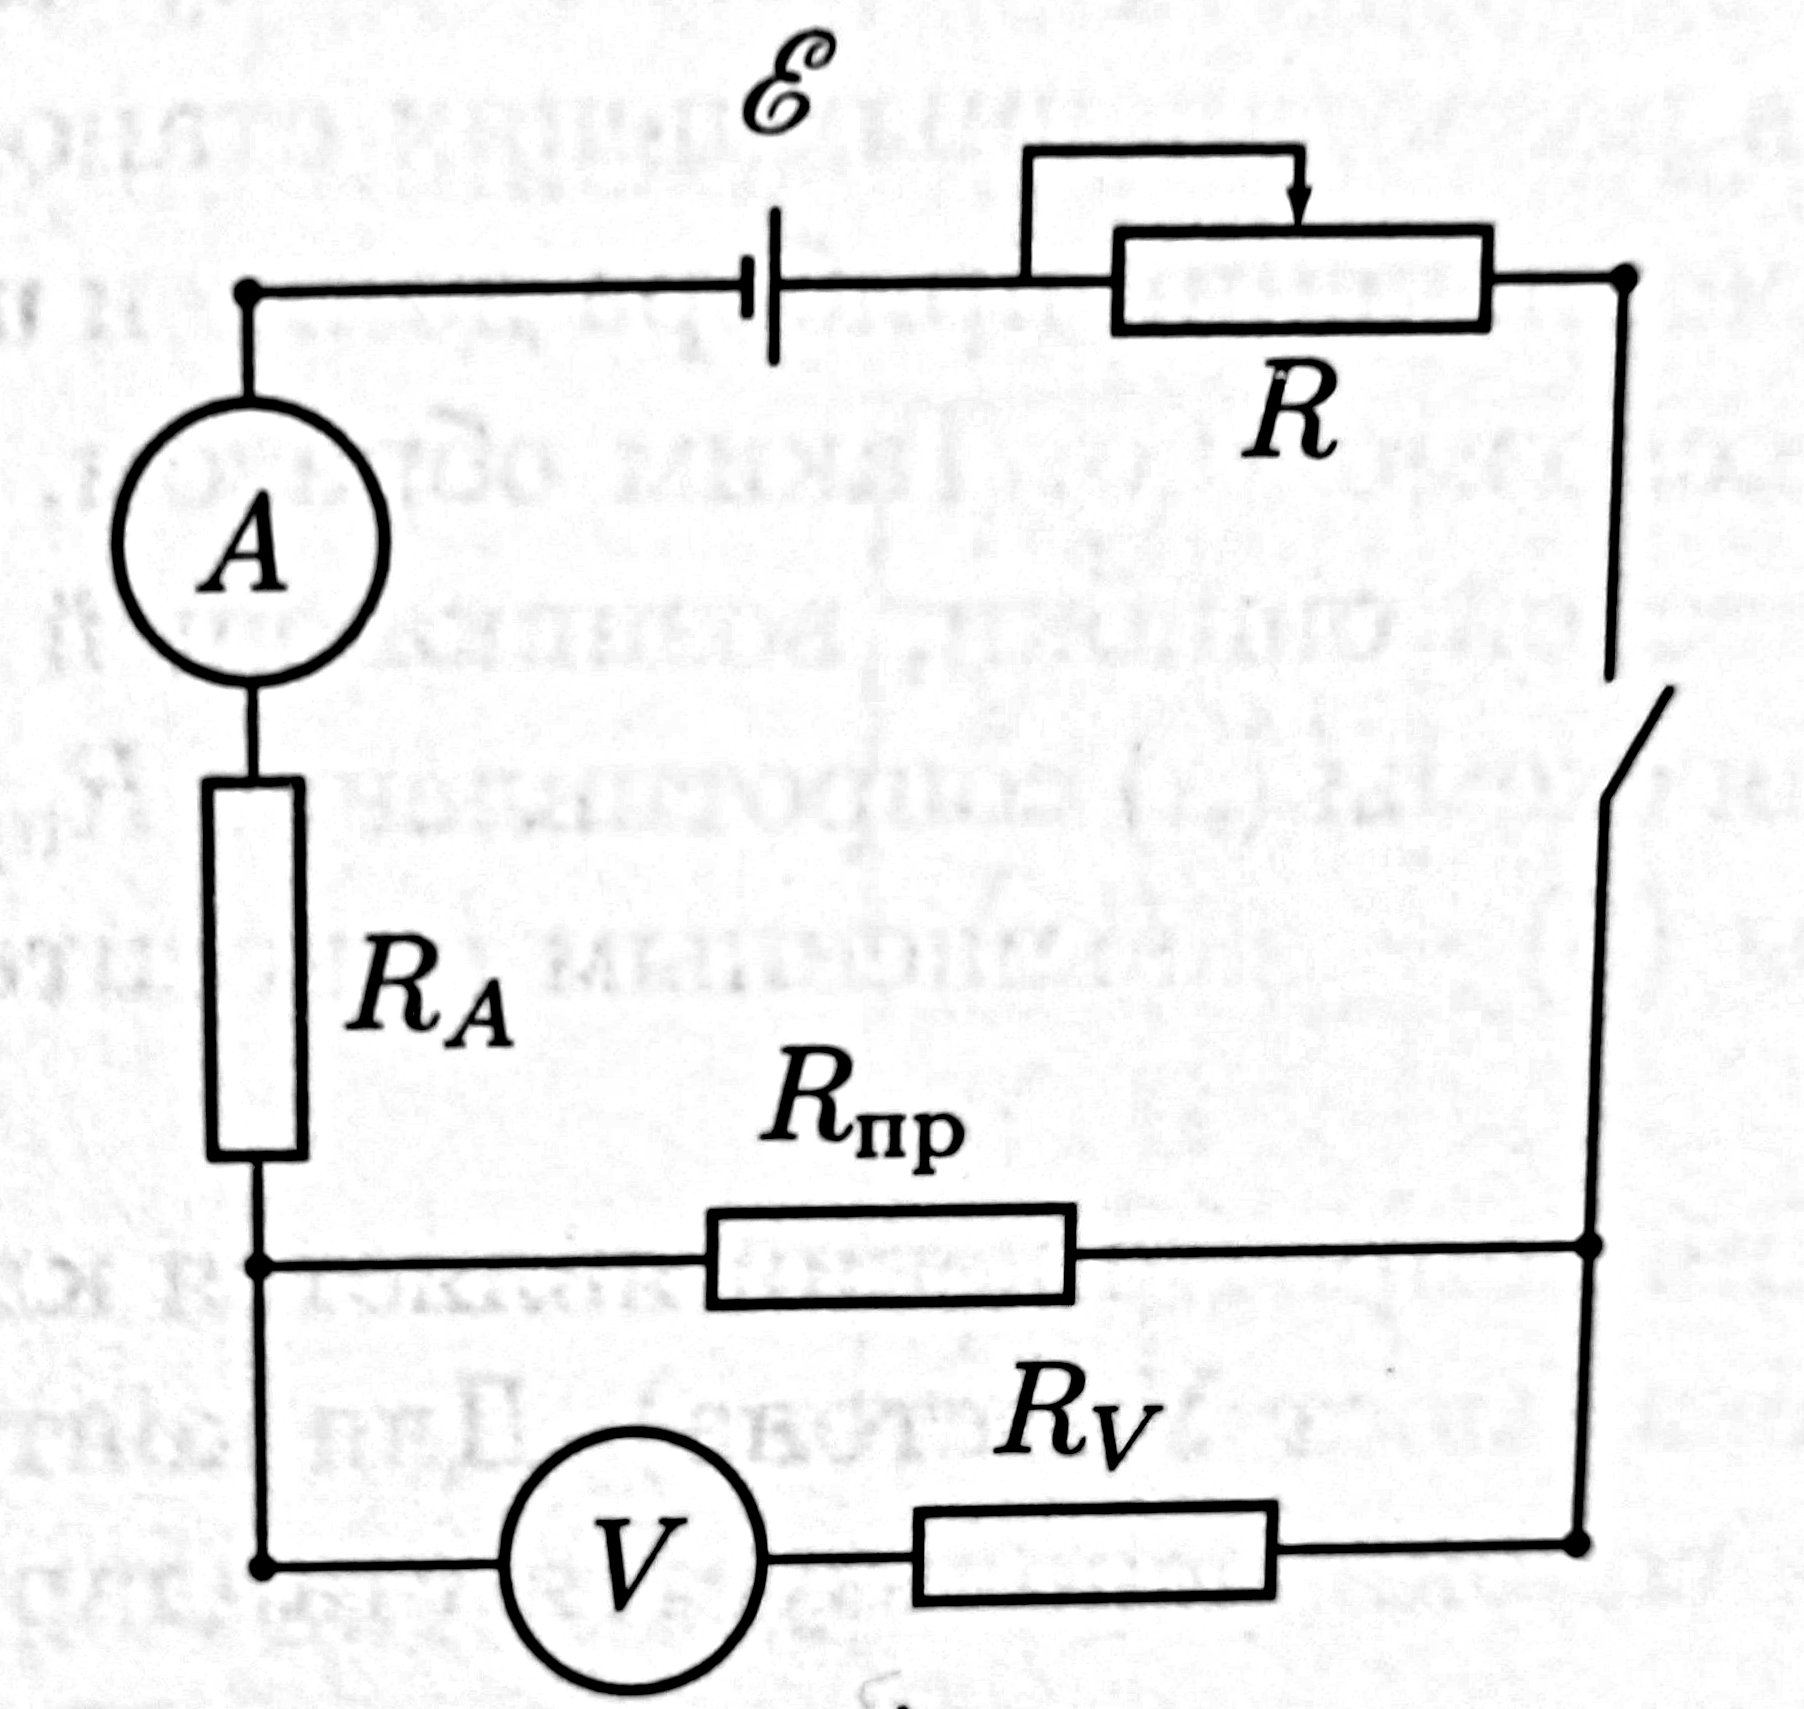
\includegraphics[width=7cm]{scheme.jpg}
	\caption{\textit{Схема цепи}}
	\label{fig:image}
\end{wrapfigure}

Согласно закону Ома напряжение $V$ и ток $I$ в образце связаны соотношением

\begin{equation}
V = RI.
\end{equation}

Для измерения напряжения и тока используем схему на \textit{рис.  \ref{fig:image}}.

\medskip

Т.к. используемый вольтметр неидеален необходимо сделать поправку на его сопротивление $R_V$.

\medskip

Показания амперметра $I_A$ и вольтметра $V_\text{В}$ связаны следующим соотношением

\begin{equation}
V_\text{В}=R^\prime I_A,
\end{equation}

\noindent где $R^\prime$ -- сопротивление параллельно соединённых проволоки и~вольтметра.

\medskip

При этом $\frac{1}{R^\prime} = \frac{1}{R_V} + \frac{1}{R}$, и $R_V \gg R, R^\prime$.\\

Таким образом, график зависимости $V_\text{В}\left(I_A\right)$ должен представлять прямую, угловой коэффициент которой есть $R^\prime$, откуда сопротивление образца может быть найдено по следующей формуле:

\begin{equation}\label{r_provoloki}
R = \dfrac{R_V R^\prime}{R_V - R^\prime} \approx R^\prime \left( 1 + \frac{R^\prime}{R_V} \right) 
\end{equation}

\section{Оборудование и экспериментальные погрешности}

\textbf{Штангенциркуль:} $\Delta_\text{шт} = \pm 0,01$ мм \\
\textbf{Микрометр:} $\Delta_\text{мкм} = \pm 0,005$ мм \\
\textbf{Вольтметр:} 

\begin{tabular}[]{|l|l|}
\hline
Система & Магнито-электрическая \\
\hline
Класс точности & 0,5 \\
\hline
Предел измерений & 0,75 мА  \\
\hline
Цена деления & $5 \cdot 10^{-3} \text{ В} = 5 \text{ мВ}$  \\
\hline
Чувствительность& 200 дел./В \\
\hline
Внутреннее сопротивление& 5 кОм  \\
\hline
Погрешность при считывании со шкалы& $\pm2,5\text{ мВ}$  \\
\hline
Максимальная погрешность по классу точности& $\pm3,75\text{ мВ}$ \\
\hline
\end{tabular}\\

\noindent \textbf{Амперметр:}

\begin{tabular}{|l|l|}
	\hline
	Система&Цифровая \\
	\hline
	Предел измерения&2 А \\
	\hline
	Разрядность дисплея& 5 ед. \\
	\hline
	Внутреннее сопротивление& $R_A = 1,4 \text{ Ом}$ \\
	\hline
\end{tabular}\\

\medskip

В диапазоне измерения $R$ от 1 до 10 Ом относительная поправка 
к сопротивлению согласно ф-ле \eqref{r_provoloki} составляет $\approx 10^{-4} \% $ (при $ R^\prime=10 \text{ Ом} $ и $ R_V = 5 \text{ кОм} $). Поэтому эта поправка пренебрежимо мала и не оказывает значительного влияния на последующие измерения. Поэтому далее будем считать, что

\begin{equation}
R\approx R^\prime
\end{equation}\\

\noindent\textbf{Мост постоянного тока P4833:}\\
\begin{tabular}{|p{8cm}|p{7cm}|}
	\hline
	Класс точности&0,1 \\
	\hline
	Разрядность магазина сопротивлений& 5 ед. \\
	\hline
	Исследуемый диапазон измерений& $ 10^{-4} - 10 \text{ Ом} $ (для множителя $ N = 10^{-2} $) \\
	\hline
	Погрешность измерений в используемом диапазоне& $\pm0,010\text{ Ом}$ \\
	\hline
\end{tabular}\\

\section{Результаты измерений и обработка данных}

\subsection{Измерение диаметра $d$ проволоки}

Измерения проводились штангенциркулем и микрометром для $N = 10$ различных участков проволоки. При измерении штангенциркулем получено $d = 0,36$ мм для всех участков. При измерении микрометром были получены следующие показания:

\begin{table}[h]
	\begin{tabular}{|l|l|l|l|l|l|l|l|l|l|l|}
		\hline
		Номер   измерения & 1    & 2    & 3    & 4    & 5    & 6    & 7    & 8    & 9    & 10   \\ \hline
		d, мм             & 0,35 & 0,36 & 0,36 & 0,35 & 0,36 & 0,36 & 0,36 & 0,35 & 0,36 & 0,36 \\ \hline
	\end{tabular}\caption{\textit{Измерение диаметра проволоки микрометром}}
\end{table}

Среднее значение диаметра $ \overline{d} = \frac{\sum d_i}{N} = 0,357 \text{ мм}$.\\

Случайная погрешность измерения $ \sigma_{\overline{d}} = \sqrt{\frac{1}{N  (N-1)}\sum(d_i-\overline{d})^2} \approx 0,001 \text{ мм}$.\\

С учётом инструментальной погрешности $ \Delta_\text{мкм} = 0,005$ мм погрешность диаметра может быть вычислена как $ \sigma^{\text{полн}}_{\overline{d}} = \sqrt{\sigma^2_{\overline{d}} + \Delta^2_{\text{мкм}}} \approx 0,005 \text{ мм}$. \\

\textit{Окончательные результаты измерения диаметра проволоки:}

\begin{itemize}
	\item Штангенциркулем: $ d = 0,36 \pm 0,01 \text{ мм}  $
	\item Микрометром:  $ \underline{0,357 \pm 0,005 \text{ мм}} \left(\varepsilon = 1,4 \%\right)  $
\end{itemize}
\subsection{Измерение сопротивления проволоки}

Результаты измерений зависимостей показания вольтметра $ V_\text{В} $ от показаний амперметра $ I_A $ в схеме на \textit{рис.  \ref{fig:image}} представлены в \textit{Таблице \ref{tab:VotI}}. Соответствующие графики зависимостей изображены на \textit{рис. \ref{graph}}.\\

Пользуясь методом наименьших квадратов, строим аппроксимирующие прямые $ V_\text{В} = \overline{R}I_A $, определяя их угловой коэффициент по формуле

\begin{equation}
\overline{R} = \frac{\langle VI \rangle}{\langle I^2 \rangle}.
\end{equation}

\begin{table}[h]
	\noindent\begin{tabular}{|p{1,6cm}|p{1cm}|p{1cm}|p{1cm}|p{1cm}|p{1cm}|p{1cm}|p{1cm}|p{1cm}|p{1cm}|p{1cm}|}
		\hline
		\multicolumn{11}{|c|}{$ l = 20 $ см}                                                                    \\ \hline
		$ V_\text{ В} $, дел. & 145    & 119    & 85     & 54     & 40    & 44     & 55     & 70     & 81     & 142    \\ \hline
		$ V_\text{ В} $, мВ      & 725    & 595    & 425    & 270    & 200   & 220    & 275    & 350    & 405    & 710    \\ \hline
		$ I_A $, мА      & 334,16 & 275,28 & 194,88 & 123,62 & 92,33 & 102,75 & 127,91 & 162,69 & 186,32 & 328,03 \\ \hline
		\multicolumn{11}{|c|}{$ l = 30 $ см}                                                                    \\ \hline
		$ V_\text{ В} $, дел. & 149    & 120    & 91     & 71     & 52    & 59     & 67     & 78     & 94     & 124    \\ \hline
		$ V_\text{ В} $, мВ      & 745    & 600    & 455    & 355    & 260   & 295    & 335    & 390    & 470    & 620    \\ \hline
		$ I_A $, мА      & 227,16 & 182,61 & 138,14 & 107,99 & 78,89 & 90,03  & 101,51 & 117,83 & 142,59 & 189,22 \\ \hline
		\multicolumn{11}{|c|}{$ l = 50 $ см}                                                                    \\ \hline
		$ V_\text{ В} $, дел. & 150    & 136    & 114    & 92     & 77    & 88     & 105    & 130    & 143    & 125    \\ \hline
		$ V_\text{ В} $, мВ      & 750    & 680    & 570    & 460    & 385   & 440    & 525    & 650    & 715    & 625    \\ \hline
		$ I_A $, мА      & 139,06 & 125,81 & 105,1  & 85,15  & 71,16 & 81,32  & 97,09  & 120,46 & 132,55 & 115,25 \\ \hline
	\end{tabular}
\caption{\textit{Зависимость $ V_\text{В} $ от $ I_A $ для разных длин проволоки $ l $.}}\label{tab:VotI}

\end{table}

Случайную погрешность определения углового коэффициента вычисляем как

\begin{equation}
\sigma^\text{сл}_R = \sqrt{\frac{1}{n-1}\left( \frac{\langle V^2\rangle}{\langle I^2 \rangle} - \overline{R}^2 \right) },
\end{equation}

где $ n = 10 $ -- число измерений.

Теперь оценим систематическую погрешность, которая возникает из-за неточности используемых приборов. Полагая, что при всех измерениях относительная погрешность неизменна, оценим погрешность вычисления частного $ R = V / I $ при максимальных значения $ V $ и $ I $:

\begin{equation}
\Delta^\text{сист}_R \approx R\sqrt{\left( \frac{\Delta_V}{V_{max}} \right)^2 + \left( \frac{\Delta_I}{I_{max}} \right)^2  }
\end{equation}

Тогда полная погрешность измерения $ R $ вычисляется следующим образом:

\begin{equation}
\sigma^\text{полн}_R = \sqrt{\left( \sigma^\text{сл}_R \right)^2 + \left( \Delta_R^\text{сист} \right)^2 }.
\end{equation}

\label{chetire}

Результаты вычислений приведены в \textit{Таблице \ref{tab:rezult}}. Там же представлены результаты измерения сопротивления при помощи моста P4833.

\begin{table}[h]
	\begin{tabular}{|l|l|l|l|l|l|l|}
		\hline
		$l$, см & $\overline{R}$, Ом & $ \sigma_R^\text{сл} $, Ом & $ \sigma_R^\text{сист} $, Ом & $ \sigma_r^\text{полн} $, Ом & $ \varepsilon, \% $ & $ R_\text{мост} $, Ом \\ \hline
		20 & 2,170 & 0,008 & 0,007 & 0,011 & 0,5 & $ (2,174 \pm 0,010) $ \\ \hline
		30 & 3,270 & 0,009 & 0,011 & 0,014 & 0,4 & $ (3,276 \pm 0,010) $ \\ \hline
		50 & 5,382 & 0,017 & 0,018 & 0,025 & 0,5 & $ (5,363 \pm 0,010) $ \\ \hline
	\end{tabular}
\caption{\textit{Результаты измерения сопротивления проволоки}}
\label{tab:rezult}
\end{table}



\begin{figure}[h!]
	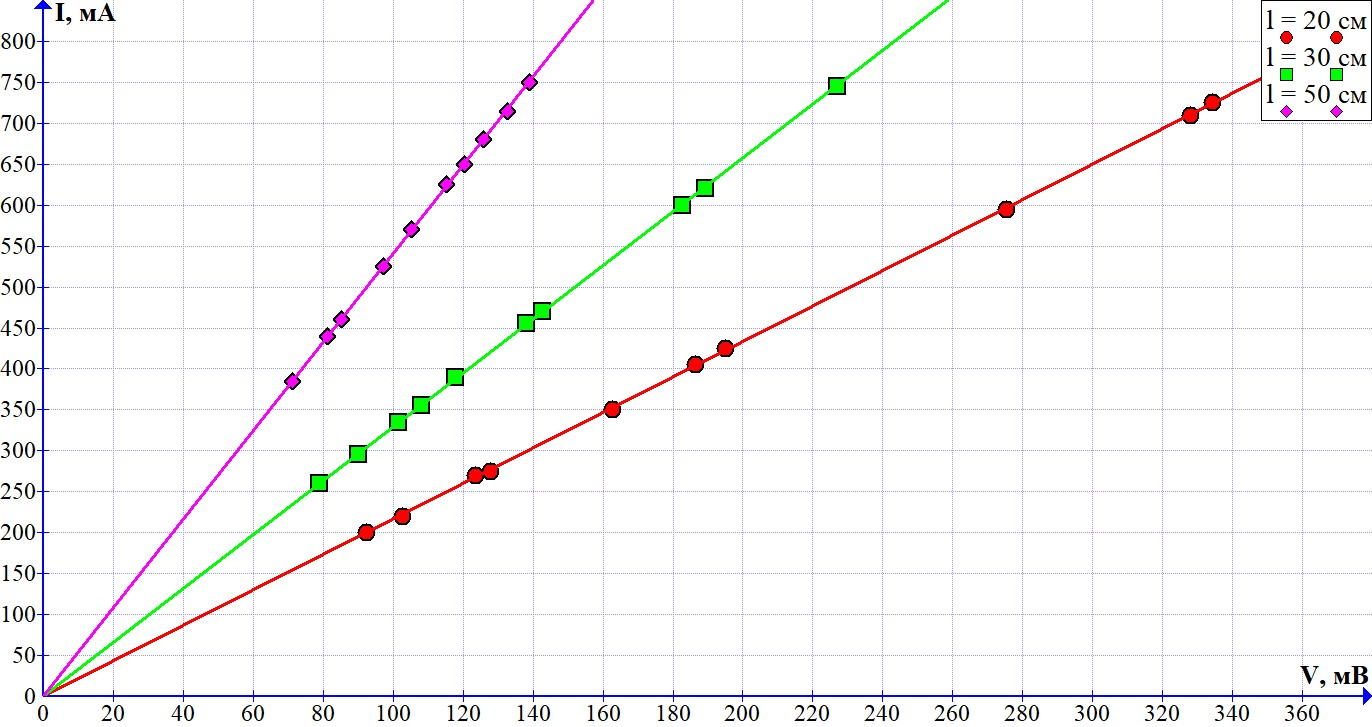
\includegraphics[width=1\linewidth]{gr.jpeg}
	\caption{\textit{Результаты измерений напряжения $ V_\text{В} $ в зависимости от тока $ I_A $ для проволок разной длины $ l $ и их линейная аппроксимация $ y=kx $.}}
	\label{graph}
\end{figure}
	
	
Таким образом, относительная погрешность измерения сопротивления достаточно мала и находится на уровне $ 0,5\% $. Также вычисленные значения сопротивления достаточно хорошо совпадают с измерениями при помощи моста.	

\subsection{Вычисление удельного сопротивления}

По формуле \eqref{1form} находим удельное сопротивление материала проволоки, используя значения, полученные в п. \ref{chetire}. Относительную погрешность вычисления $ \rho $ определяем по следующей формуле и заносим результаты в \textit{таблицу \ref{rezi}}:

\begin{equation}
\sigma_\rho = \rho \sqrt{\left( \frac{\sigma_R}{R}  \right)^2 + \left( 2 \frac{\sigma_d}{d} \right) ^2 }.
\end{equation}

\begin{table}[h]

	\begin{tabular}{|l|l|l|l|}
		\hline
		& $ \rho , \text{Ом} \cdot \text{мм}^2 / \text{м} $   & $ \sigma_p, \text{Ом} \cdot \text{мм}^2 / \text{м} $ & $ \varepsilon_\rho, \% $   \\ \hline
		$l$ = 20 см & 1,086 & 0,032 & 3,0 \\ \hline
		$l$ = 30 см & 1,092 & 0,032 & 2,9 \\ \hline
		$l$ = 50 см & 1,079 & 0,032 & 2,9 \\ \hline
	\end{tabular}
	\caption{\textit{Результат измерения удельного сопротивления}}\label{rezi}
\end{table}


Усредняя результаты трёх опытов, окончательно получаем:

\begin{equation}
\overline{\rho} = \underline{\left( 1,086 \pm 0,032 \right) \text{Ом} \cdot \text{мм}^2 / \text{м}} \left( \varepsilon_\rho = 2,9 \% \right) 
\end{equation}

\section{Обсуждение результатов и выводы}

В ходы работы было получено значение удельного сопротивления нихромовой проволоки с точностью $ \sim 3 \% $. Табличные значения для нихрома лежат в диапазоне $ 0,99 \dots 1,12 \text{ Ом} \cdot \text{мм}^2 / \text{м}$ в зависимости от состава различных сплавов. Измеренные значения $ \rho = \left( 1,086 \pm 0,032 \right) \text{Ом} \cdot \text{мм}^2 / \text{м} $ попадают в нужный диапазон, однако они не позволяют точно определить марку сплава.

\medskip

\noindent Точность измерения удельного сопротивления $ \rho $ существенно ограничивается измерением
диаметра проволоки. Поскольку случайная ошибка измерения диаметра оказалась меньше
цены деления прибора (микрометра), уточнение значения диаметра за счет многократных измерений невозможно. По той же причине не удалось проверить, насколько однородной является проволока по сечению.
	
	
	
	
	
	
\end{document}